\chapter{Image Matching and Motion Estimation}
\section{Image matching}
找两个图像之间点与点的关系. 
\begin{figure}[H]
    \centering
    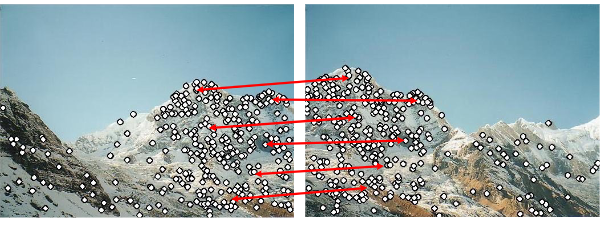
\includegraphics[width=0.38\textwidth]{Lec5/matching}
    \caption{Image matching}
\end{figure}

Application: 几乎所有CV的问题都可以转换为此问题. 
\begin{enumerate}
    \item Image alignment
    \item 3D reconstruction
    \item Motion tracking
    \item Object recognition
    \item Indexing and database retrieval
    \item Robot navigation
    \item ... other
\end{enumerate}

Main Components of Feature matching
\begin{enumerate}
    \item Detection(检测): Identify the interest points.
    \item Description(描述): Extract(提取) vector feature descriptor(描述子) surrounding each interest point.
    \item Matching: Determine correspondence between descriptors in two views. 
\end{enumerate}

\subsection{Detection}
寻找点的唯一性.
\subsubsection{Local measures of uniqueness}
    衡量的是点的领域. 唯一性可以看作移动这个领域后的变化.
    \begin{figure}[H]
        \centering
        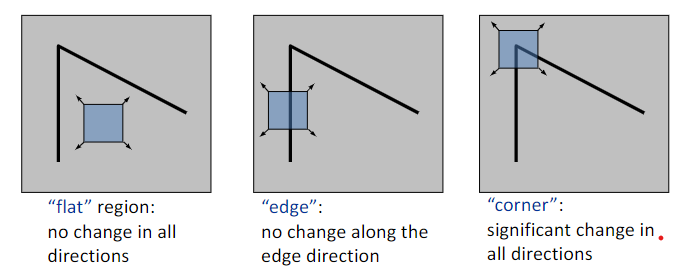
\includegraphics[width=0.33\textwidth]{Lec5/uniqueness}
        \caption{uniqueness}
    \end{figure}

    数学上可以用梯度衡量, 坐标描述的是领域中梯度的分布. 
    \begin{figure}[H]
        \centering
        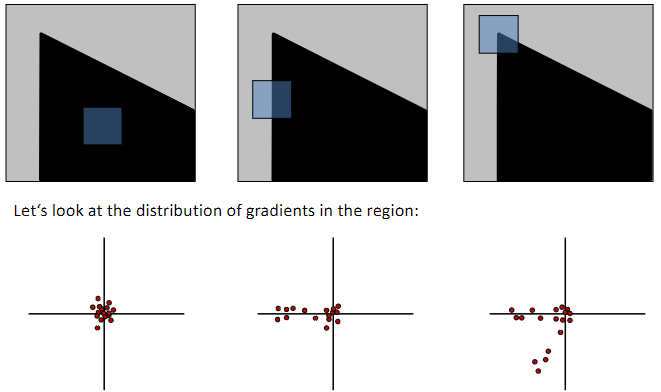
\includegraphics[width=0.33\textwidth]{Lec5/measure uniqueness}
        \caption{measure uniqueness}
    \end{figure}

\paragraph{Principal Component Analysis(主成分分析)}
第一个主成分是方差最大的方向, 第二个主成分是与第一个主成分垂直的方差最大的方向. 
\begin{figure}[H]
    \centering
    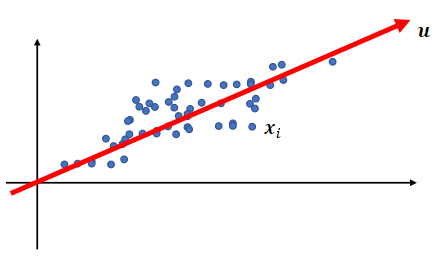
\includegraphics[width=0.33\textwidth]{Lec5/PCA}
    \caption{PCA}
\end{figure}

\paragraph{Corner detection}
\begin{enumerate}
    \item Compute the covariance matrix(协方差矩阵) at each point. 
    \begin{align*}
        H&=\sum_{u,v} w(u,v)\begin{bmatrix}
            I_x^2 & I_xI_y\\
            i_xI_y & I_y^2
        \end{bmatrix}\\
        I_x&=\frac{\partial f}{\partial x}\\
        I_y&=\frac{\partial f}{\partial  y}\\
        w(u,v)&\text{ is typically Gaussian weights}
    \end{align*}
    \item Compute eigenvalues(特征值).
    \begin{align*}
        H&=\begin{bmatrix}
            a&b\\c&d
        \end{bmatrix}\\
        \lambda_{\pm}&=\frac{1}{2}((a+d)\pm \sqrt{4bc+(a-d)^2})
    \end{align*}
    \item Classify points using eigenvalues of $H$:
\end{enumerate}

\begin{figure}[H]
    \centering
    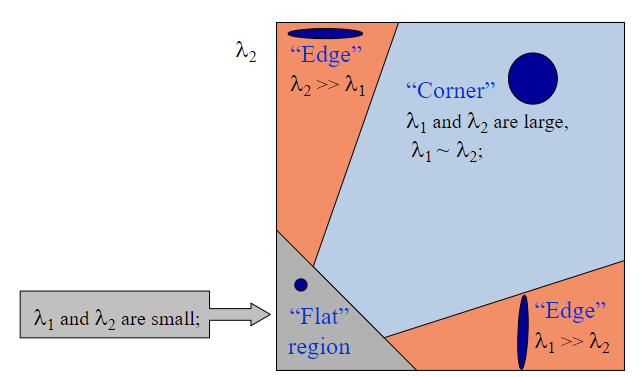
\includegraphics[width=0.38\textwidth]{Lec5/Corner detection}
    \caption{Corner detection}
\end{figure}


\paragraph{The Harris operator}

算特征值开销太大, Harris corner detector用以来代替
\begin{align*}
    f&=\frac{\lambda_1\lambda_2}{\lambda_1+\lambda_2}=\frac{det(H)}{trace(H)}\\
    det(\begin{bmatrix}
        a&b\\c&d
    \end{bmatrix})&=ad-bc\text{为行列式}\\
    trace(\begin{bmatrix}
        a&b\\c&d
    \end{bmatrix})&=a+d\text{为迹,即对角线之和(需对称矩阵)}
\end{align*}

f叫做角点检测的响应值(corner response)

Harris detector
\begin{enumerate}
    \item Compute derivatives(梯度/导数) at each pixel
    \item Compute covariance matrix H(协方差矩阵) in a Gaussian window around each pixel
    \item Compute corner response(响应值) function f
    \item Threshold f
    \item Find local maxima of response function(nonmaximum suppression)
\end{enumerate}

但要如何保证两幅图检测出来点的重复性(repeatable)?

因此想要f对图像的变换具有不变性(invariant).

\paragraph{Harris detector: Invariance properties}
image transformations
\begin{enumerate}
    \item photometric: 亮度变换
    \item Geometric
    \begin{enumerate}
        \item 平移
        \item 旋转
        \item 缩放
    \end{enumerate}
\end{enumerate}

Harris detector(讨论对应点的响应值)
\begin{enumerate}
    \item photometric transformation $I \longrightarrow  aI+b$
    \begin{enumerate}
        \item $I \longrightarrow  I+b$梯度不变, f不变
        \item $I \longrightarrow  aI$梯度改变, f改变
    \end{enumerate}

    所以是部分改变
    \item  Image translation(平移) f不变
    \item Image rotation(旋转) f不变
    \item Scaling(缩放) f改变(图像变大, 领域中梯度改变了)
\end{enumerate}

如何正确选择窗口大小?逝()

不同窗口扫下来, 最大f应该一样, 但尺度不同, 所以选最大的.用 image pyramid 缩小图像, 用相同的领域去扫这个 pyramid, 以此确定最好的尺度. 

\subsubsection{Blob detector(斑点检测)}
斑点有较大的二阶导数(极值点)

用拉普拉斯算子(Laplacian)$\Delta=\nabla^2$, $I_{xx}+I_{yy}$卷积计算, 
\begin{align*}
    \nabla^2=\frac{\partial^2 }{\partial x^2}+\frac{\partial^2 }{\partial y^2}
\end{align*}

\paragraph{Laplacian of Gaussian}
因为其对噪声十分敏感, 所以用卷积核 Laplacian of Gaussian (LoG) filter 来计算, 以抑制噪声.
\begin{figure}[H]
    \centering
    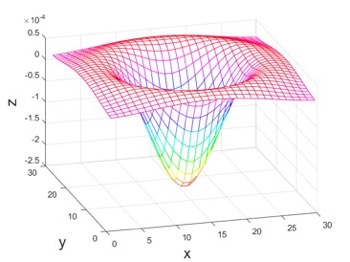
\includegraphics[width=0.22\textwidth]{Lec5/LOG}
    \caption{Laplacian of Gaussian}
\end{figure}
\begin{align*}
    \nabla^2(f*G)&=f*\nabla^2G\\
    \therefore\text{use LoG } \nabla^2 G&=\frac{\partial^2 G}{\partial x^2}+\frac{\partial^2 G}{\partial y^2}\\
    G& \text{ is 2D Gaussian function}
\end{align*}

LoG尺度(scale)取决于Gaussian 的$\sigma$.
\begin{figure}[H]
    \centering
    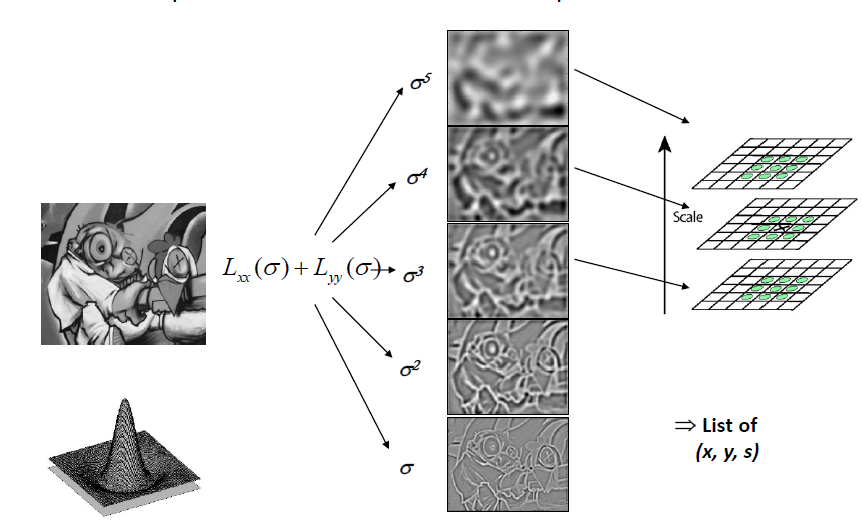
\includegraphics[width=0.22\textwidth]{Lec5/Scale of LoG}
    \caption{Scale of LoG}
\end{figure}


尺度选择: 用不同$\sigma$去试(), 也是找最大的f值的$\sigma$.

\paragraph{Difference-of-Gaussian(DoG)} $\nabla^2 G_{\sigma}\approx G_{\sigma_1}-G_{\sigma_2}$(LoG可用两个Gaussian的差作近似) 

Best approximation when $\sigma_1=\frac{\sigma}{\sqrt{2}}, \sigma_2=\sqrt{2}\sigma$.

不同尺度下, 用不同$\sigma$计算再两两相减得出. 
\begin{figure}[H]
    \centering
    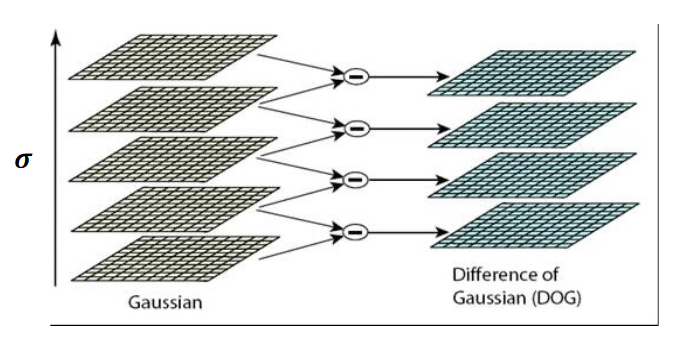
\includegraphics[width=0.22\textwidth]{Lec5/Scale of DoG}
    \caption{Scale of DoG}
\end{figure}

DoG一般比LoG高效(Gaussian比较快)

\subsection{Description}

\subsubsection{Feature descriptors(构造描述子)}
一般是个vector(向量)
\paragraph{Describe an image patch} 描述像素块, 直接把一个像素块表示为一个向量. (这并不好, 因为其不变性非常差.)

\paragraph{SIFT descriptor}Scale Invariant Feature Transform (SIFT), 最常用. 本质上是对 patch 内图像梯度的统计. SIFT就是用patch内梯度朝向分布作描述子. 
\begin{figure}[H]
    \centering
    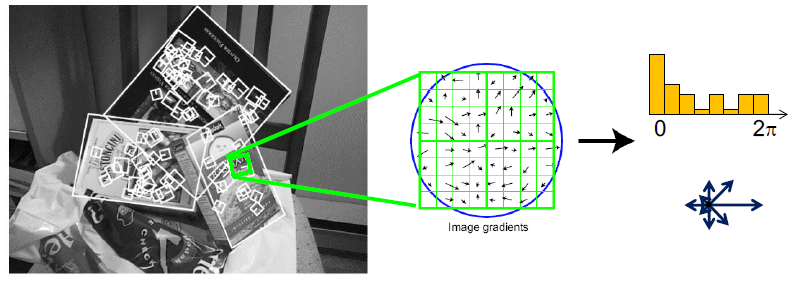
\includegraphics[width=0.38\textwidth]{Lec5/SIFT}
    \caption{SIFT}
\end{figure}

\subparagraph{不变性}
\begin{enumerate}
    \item 对亮度有较好不变性
    \item 缩放有不变性(因为其特殊检测阶段的手段确定了缩放不变, 而不是其本身有不变性)
    \item 旋转有不变性 (Orientation Normalization, 对朝向进行了归一化)
    \begin{enumerate}
        \item Compute orientation histogram(求朝向)
        \item Select dominant orientation(选择主朝向)
        \item Normalize: rotate to fixed orientation(归一化)
    \end{enumerate}
\end{enumerate}

\subparagraph{流程}
\begin{enumerate}
    \item Run DoG detector
    \begin{enumerate}
        \item Find maxima in location/scale space
        \item Remove edge points
    \end{enumerate}
    \item Find dominate orientation(朝向归一化)
    \item For each (x,y,scale,orientation), create descriptor
\end{enumerate}
\subsubsection{一些其他检测器与描述子 detectors and descriptors}
SIFT已经是传统的效果的极限了(不传统指神经网络)

其他有些是为了更快之类的. 
\begin{enumerate}
    \item HOG: Histogram of oriented gradients
    \begin{itemize}
        \item  Dalal \& Triggs, 2005
    \end{itemize}
    \item SURF: Speeded Up Robust Features
    \begin{itemize}
        \item  Herbert Bay, Andreas Ess, Tinne Tuytelaars, Luc Van Gool, "SURF: Speeded Up Robust Features", Computer Vision and Image Understanding (CVIU), Vol. 110, No. 3, pp. 346--359, 2008
    \end{itemize}
    \item FAST (corner detector)
    \begin{itemize}
        \item  Rosten. Machine Learning for High-speed Corner Detection, 2006.
    \end{itemize}
    \item ORB: an efficient alternative to SIFT or SURF
    \begin{itemize}
        \item  Ethan Rublee, Vincent Rabaud, Kurt Konolige, Gary R. Bradski: ORB: An efficient alternative to SIFT or SURF. ICCV 2011
    \end{itemize}
    \item Fast Retina Key- point (FREAK)
    \begin{itemize}
        \item  A. Alahi, R. Ortiz, and P. Vandergheynst. FREAK: Fast Retina Keypoint. In IEEE Conference on Computer Vision and Pattern Recognition, 2012. CVPR 2012
        Open Source Award Winner.
    \end{itemize}
\end{enumerate}


\subsection{Matching}

\subsubsection{Feature distance}
用距离衡量相似$\left\| f_1-f_2\right\|$, 但如果存在重复会WA.
\begin{figure}[H]
    \centering
    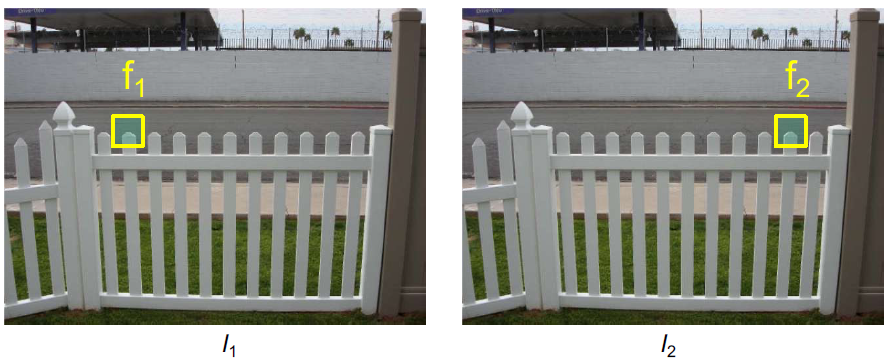
\includegraphics[width=0.38\textwidth]{Lec5/Feature distance}
    \caption{Feature distance}
\end{figure}

\paragraph{Ratio test} 
Ratio score=$\frac{\left\| f_1-f_2\right\|}{\left\| f_1-f'_2\right\|}$, 奇异点比值为1, 这个点就不太好, 那就不要了. 
\begin{figure}[H]
    \centering
    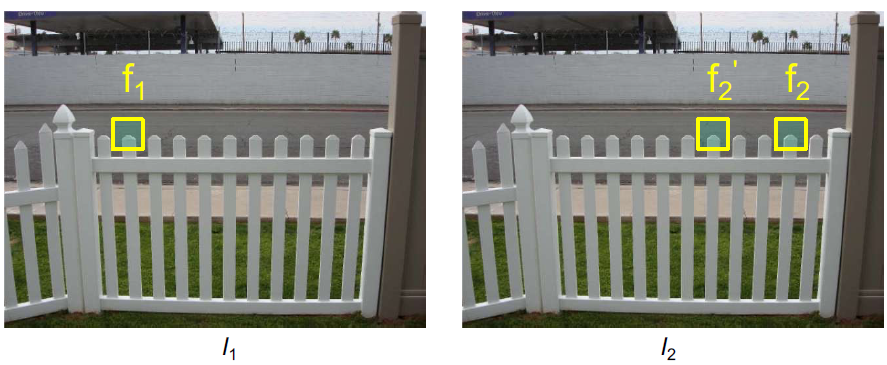
\includegraphics[width=0.38\textwidth]{Lec5/Ratio test}
    \caption{Ratio test}
\end{figure}

\paragraph{Mutual nearest neighbor}(双向最近邻)
双向寻找, 都是最接近的才是最接近的. 如果两次不一样, 那就不要这个点了. 

\subsection{Deep learning for feature matching}
训练网络来解决(), 后面讲.
\begin{figure}[H]
    \centering
    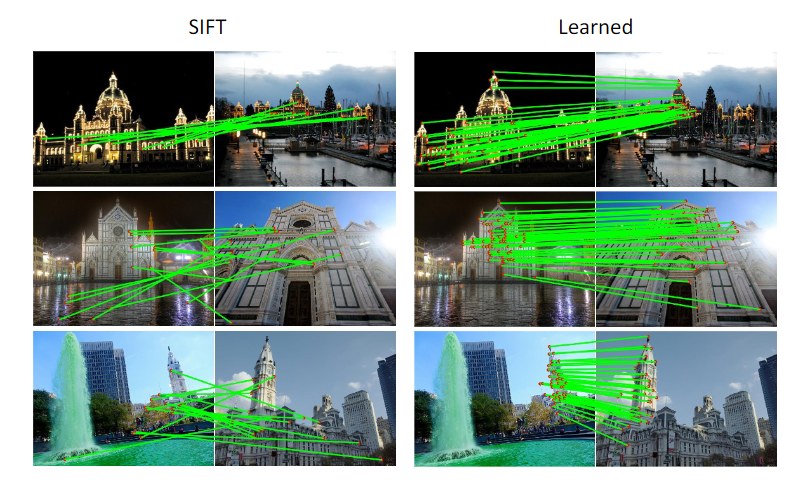
\includegraphics[width=0.44\textwidth]{Lec5/SIFTvsLearned}
    \caption{SIFT vs Learned}
\end{figure}

\section{Motion Estimation}
视频中相邻帧的运动关系. 

\subsection{Seeing motion from a static picture}
一些奇怪的图, 看着图在动, 其实是人眼在动, 导致看到的图在动. 一般运动都是看亮度有没有改变. 
\begin{figure}[H]
    \centering
    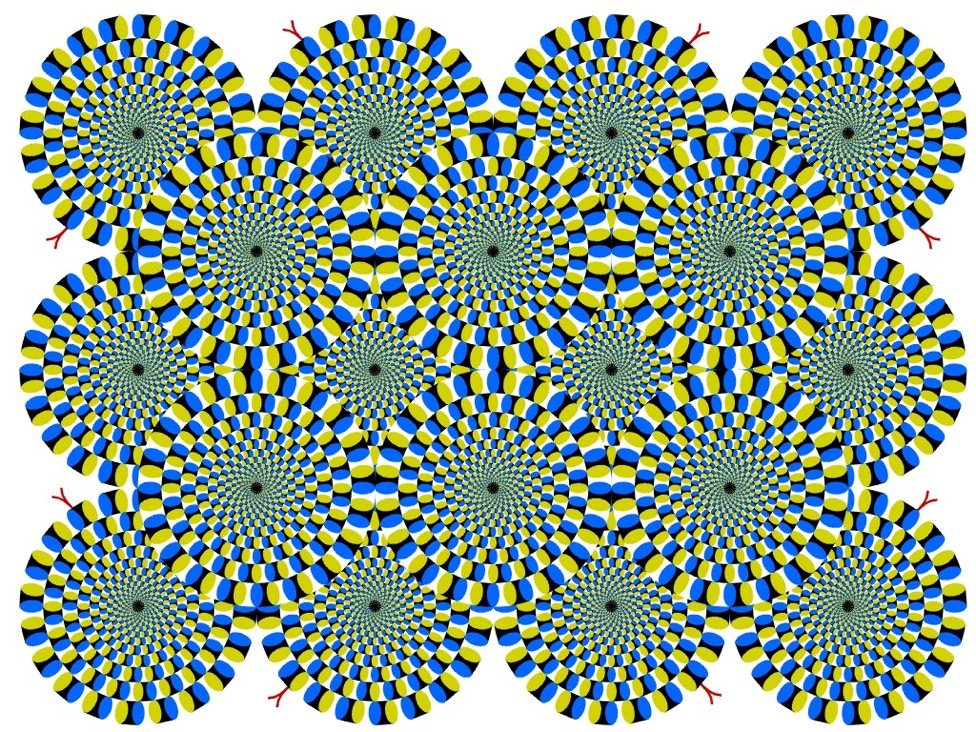
\includegraphics[width=0.44\textwidth]{Lec5/Seeing motion from a static picture}
    \caption{a static picture}
\end{figure}

\subsection{The cause of motion}
\begin{enumerate}
    \item 场景中物体运动.
    \item 相机运动.
    \item 相机与场景一起运动.
    \item 场景相机都不动, 但光线变化.(会影响运动检测)
\end{enumerate}

\subsection{Motion estimation problems}
\begin{enumerate}
    \item Feature-tracking: 跟踪每个特征点在每一帧的位置. (稀疏)
    \item Optical flow(光流): 恢复图像中每一个像素的运动. (稠密, 本质上是个向量场, 表示像素的移动)
\end{enumerate}

\subsection{Lucas-Kanade method}
 
\subsubsection{Motion estimation}
把图像记为$I(x,y,t)$.

有$I(x,y,t)$与$I(x,y,t+1)$, 求解位移. 即通过第一张图位置估计运动以此求解第二张图的位置, 本质上是求解每个点对应的平移向量. 

\subsubsection{Lucas-Kanade的假设}
\begin{enumerate}
    \item Small motion: points do not move very far(前后帧点运动较小)
    \item Brightness constancy: same point looks the same in every frame(前后帧亮度值不会有太大变化)
    \item Spatial coherence(空间连续性): points move like their neighbors(相邻点运动会比较一致)
\end{enumerate}

\subsubsection{求解}
\begin{figure}[H]
    \centering
    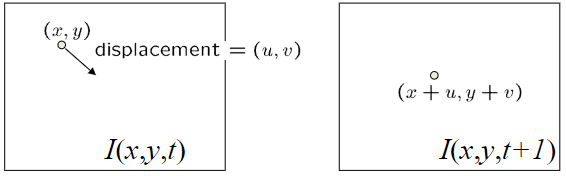
\includegraphics[width=0.44\textwidth]{Lec5/The brightness constancy}
    \caption{The brightness constancy}
\end{figure}

要求解u与v

Brightness Constancy Equation:
\begin{align*}
    I(x,y,t)&=I(x+u,y+v,t+1)\\
\end{align*}

Taylor expansion assuming small motion:($I_x$是图像关于x的导数, $I_t$用关于时间的两次的变化做差得到)
\begin{align*}
    I(x+u,y+v,t+1)&\approx I(x,y,t)+I_xu+I_yv+I_t\\
    I(x+u,y+v,t+1)-I(x,y,t)&=I_xu+I_yv+I_t\\
    \therefore I_xu+I_yv+I_t&\approx 0\\
    \therefore \nabla I \begin{bmatrix}u\\v\end{bmatrix}+I_t&=0
\end{align*}

(方程数量不足, 那么方程无法确定在哪? 自由度在何处?)若$(u,v)$满足此方程, $\exists u',v'$, 有$\nabla I \begin{bmatrix}u'\\v'\end{bmatrix}=0$, 则$(u+u',v+v')$也满足此方程. 所以垂直此方向的移动是确定不了的.

\paragraph{The aperture problem} 孔径问题, 只看局部是确定不了运动的. 

\begin{figure}[H]
    \centering
    \begin{subfigure}{0.38\textwidth}
        \centering
        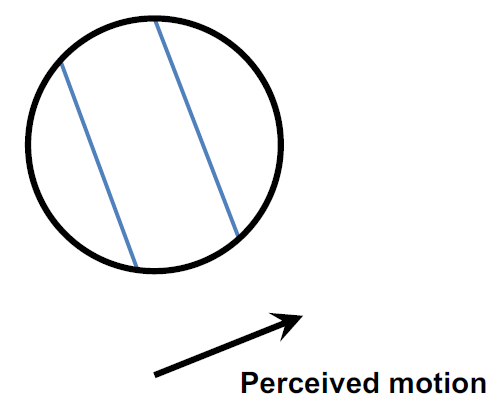
\includegraphics[width=\textwidth]{Lec5/aperture problem1}
        \caption{pre}
    \end{subfigure}
    \begin{subfigure}{0.38\textwidth}
        \centering
        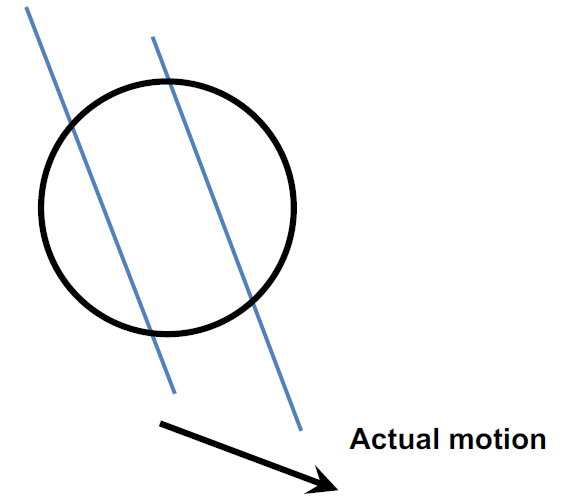
\includegraphics[width=\textwidth]{Lec5/aperture problem2}
        \caption{real}
    \end{subfigure}
    \caption{The aperture problem}
\end{figure}

Spatial coherence, 取周围的点联立建方程求解$u_i$,$v_i$. 假设周围的点$(u,v)$相同. eg:$5\times 5$共25点, 即
\begin{align*}
    \begin{bmatrix}
        I_x(p_1)& I_y(p_1)\\
        I_x(p_2)& I_y(p_2)\\
        \vdots & \vdots \\
        I_x(p_{25})& I_y(p_{25})
    \end{bmatrix}\begin{bmatrix}
        u\\v
    \end{bmatrix}&=-\begin{bmatrix}
        I_t(p_1)\\
        I_t(p_2)\\
        \vdots\\
        I_t(p_{25})
    \end{bmatrix}\\
    \underset{25\times 2}{A} \quad \underset{2\times 1}{d}&=\underset{25\times 1}{b}
\end{align*}

不一定要完全相等, 就是求$\min_d \left\| Ad-b \right\|^2$, 即求解
\begin{align*}
    (A^TA)d&=A^Tb\\
    \begin{bmatrix}
        \sum I_xI_x & \sum I_xI_y\\
        \sum I_xI_y & \sum I_yI_y
    \end{bmatrix}\begin{bmatrix}
        u\\v
    \end{bmatrix}&=\begin{bmatrix}
        \sum I_xI_t\\
        \sum I_yI_t
    \end{bmatrix}
\end{align*}

$A^TA$为领域内梯度的协方差矩阵, 但当$A^TA$不满秩无唯一解, 所以要求$\lambda_1$与$\lambda_2$不为0, 最好都比较大, 这样求逆会稳定一些. (与Harris corner detector相似, 所以角点是比较好跟踪的点)

\subsubsection{Errors in Lukas-Kanade}
当假设被违反就会产生很大的误差
\begin{enumerate}
    \item Brightness constancy is not satisfied.(光照巨变)
    \item The motion is not small(有东西快速乱窜)
    \item A point does not move like its neighbors(边缘的点/特别小的物体)
\end{enumerate}

\paragraph{Revisiting the small motion assumption}
可以减小分辨率缓解此假设的违反.

\paragraph{Coarse-to-fine optical flow estimation}从粗到细的光流估计.

根据上一层光流估计的结果改变下一层让其更满足小运动假设. (Image warping)
\begin{figure}[H]
    \centering
    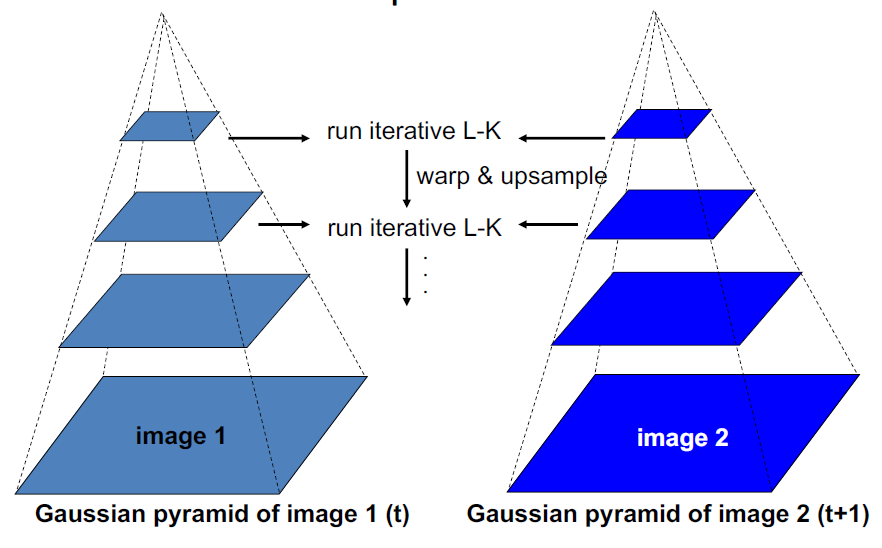
\includegraphics[width=0.44\textwidth]{Lec5/Coarse-to-fine}
    \caption{Coarse-to-fine}
\end{figure}


\subsection{光流可视化}Flow quality evaluation

用HVS颜色表示光流的方向, 大小为强度. 

常用数据集: Middlebury flow page

\subsection{Leaderbord}

来自 paperswithcode.com 

\begin{figure}[H]
    \centering
    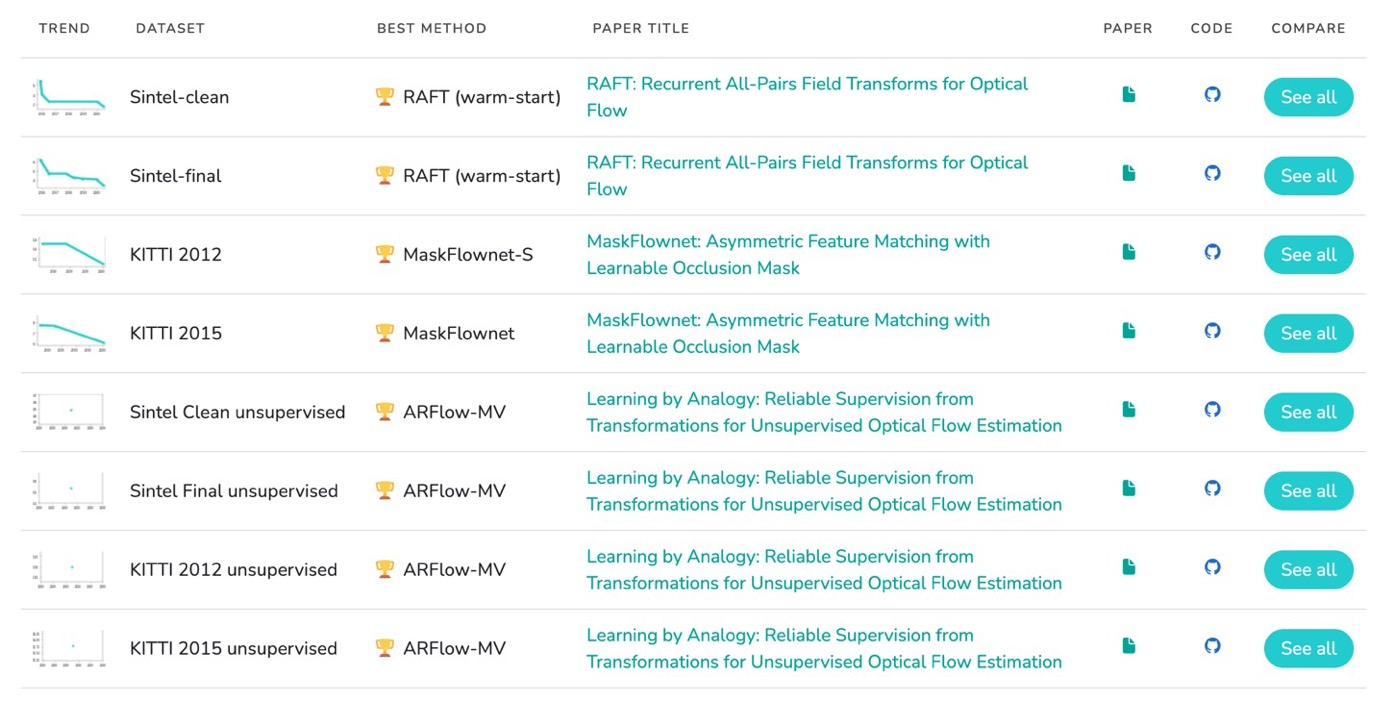
\includegraphics[width=0.65\textwidth]{Lec5/Leaderbord}
    \caption{Leaderbord}
\end{figure}

虽用DL, 但思想来自经典方法. 

\subsection{应用}
\begin{enumerate}
    \item Video stabilization(去抖动, 因为所有像素的运动多半是相机运动)
    \item Video 压缩(用光流压缩信息)
    \item Video denoising(去噪, 把滤波扩展到时序)
\end{enumerate}
